% Options for packages loaded elsewhere
\PassOptionsToPackage{unicode}{hyperref}
\PassOptionsToPackage{hyphens}{url}
\PassOptionsToPackage{dvipsnames,svgnames,x11names}{xcolor}
%
\documentclass[
  12pt]{article}

\usepackage{amsmath,amssymb}
\usepackage{iftex}
\ifPDFTeX
  \usepackage[T1]{fontenc}
  \usepackage[utf8]{inputenc}
  \usepackage{textcomp} % provide euro and other symbols
\else % if luatex or xetex
  \usepackage{unicode-math}
  \defaultfontfeatures{Scale=MatchLowercase}
  \defaultfontfeatures[\rmfamily]{Ligatures=TeX,Scale=1}
\fi
\usepackage{lmodern}
\ifPDFTeX\else  
    % xetex/luatex font selection
\fi
% Use upquote if available, for straight quotes in verbatim environments
\IfFileExists{upquote.sty}{\usepackage{upquote}}{}
\IfFileExists{microtype.sty}{% use microtype if available
  \usepackage[]{microtype}
  \UseMicrotypeSet[protrusion]{basicmath} % disable protrusion for tt fonts
}{}
\makeatletter
\@ifundefined{KOMAClassName}{% if non-KOMA class
  \IfFileExists{parskip.sty}{%
    \usepackage{parskip}
  }{% else
    \setlength{\parindent}{0pt}
    \setlength{\parskip}{6pt plus 2pt minus 1pt}}
}{% if KOMA class
  \KOMAoptions{parskip=half}}
\makeatother
\usepackage{xcolor}
\setlength{\emergencystretch}{3em} % prevent overfull lines
\setcounter{secnumdepth}{5}
% Make \paragraph and \subparagraph free-standing
\makeatletter
\ifx\paragraph\undefined\else
  \let\oldparagraph\paragraph
  \renewcommand{\paragraph}{
    \@ifstar
      \xxxParagraphStar
      \xxxParagraphNoStar
  }
  \newcommand{\xxxParagraphStar}[1]{\oldparagraph*{#1}\mbox{}}
  \newcommand{\xxxParagraphNoStar}[1]{\oldparagraph{#1}\mbox{}}
\fi
\ifx\subparagraph\undefined\else
  \let\oldsubparagraph\subparagraph
  \renewcommand{\subparagraph}{
    \@ifstar
      \xxxSubParagraphStar
      \xxxSubParagraphNoStar
  }
  \newcommand{\xxxSubParagraphStar}[1]{\oldsubparagraph*{#1}\mbox{}}
  \newcommand{\xxxSubParagraphNoStar}[1]{\oldsubparagraph{#1}\mbox{}}
\fi
\makeatother


\providecommand{\tightlist}{%
  \setlength{\itemsep}{0pt}\setlength{\parskip}{0pt}}\usepackage{longtable,booktabs,array}
\usepackage{calc} % for calculating minipage widths
% Correct order of tables after \paragraph or \subparagraph
\usepackage{etoolbox}
\makeatletter
\patchcmd\longtable{\par}{\if@noskipsec\mbox{}\fi\par}{}{}
\makeatother
% Allow footnotes in longtable head/foot
\IfFileExists{footnotehyper.sty}{\usepackage{footnotehyper}}{\usepackage{footnote}}
\makesavenoteenv{longtable}
\usepackage{graphicx}
\makeatletter
\def\maxwidth{\ifdim\Gin@nat@width>\linewidth\linewidth\else\Gin@nat@width\fi}
\def\maxheight{\ifdim\Gin@nat@height>\textheight\textheight\else\Gin@nat@height\fi}
\makeatother
% Scale images if necessary, so that they will not overflow the page
% margins by default, and it is still possible to overwrite the defaults
% using explicit options in \includegraphics[width, height, ...]{}
\setkeys{Gin}{width=\maxwidth,height=\maxheight,keepaspectratio}
% Set default figure placement to htbp
\makeatletter
\def\fps@figure{htbp}
\makeatother

\addtolength{\oddsidemargin}{-.5in}%
\addtolength{\evensidemargin}{-1in}%
\addtolength{\textwidth}{1in}%
\addtolength{\textheight}{1.7in}%
\addtolength{\topmargin}{-1in}%
\usepackage{booktabs}
\usepackage{longtable}
\usepackage{array}
\usepackage{multirow}
\usepackage{wrapfig}
\usepackage{float}
\usepackage{colortbl}
\usepackage{pdflscape}
\usepackage{tabu}
\usepackage{threeparttable}
\usepackage{threeparttablex}
\usepackage[normalem]{ulem}
\usepackage{makecell}
\usepackage{xcolor}
\makeatletter
\@ifpackageloaded{caption}{}{\usepackage{caption}}
\AtBeginDocument{%
\ifdefined\contentsname
  \renewcommand*\contentsname{Table of contents}
\else
  \newcommand\contentsname{Table of contents}
\fi
\ifdefined\listfigurename
  \renewcommand*\listfigurename{List of Figures}
\else
  \newcommand\listfigurename{List of Figures}
\fi
\ifdefined\listtablename
  \renewcommand*\listtablename{List of Tables}
\else
  \newcommand\listtablename{List of Tables}
\fi
\ifdefined\figurename
  \renewcommand*\figurename{Figure}
\else
  \newcommand\figurename{Figure}
\fi
\ifdefined\tablename
  \renewcommand*\tablename{Table}
\else
  \newcommand\tablename{Table}
\fi
}
\@ifpackageloaded{float}{}{\usepackage{float}}
\floatstyle{ruled}
\@ifundefined{c@chapter}{\newfloat{codelisting}{h}{lop}}{\newfloat{codelisting}{h}{lop}[chapter]}
\floatname{codelisting}{Listing}
\newcommand*\listoflistings{\listof{codelisting}{List of Listings}}
\makeatother
\makeatletter
\makeatother
\makeatletter
\@ifpackageloaded{caption}{}{\usepackage{caption}}
\@ifpackageloaded{subcaption}{}{\usepackage{subcaption}}
\makeatother

\ifLuaTeX
  \usepackage{selnolig}  % disable illegal ligatures
\fi
\usepackage[]{natbib}
\bibliographystyle{agsm}
\usepackage{bookmark}

\IfFileExists{xurl.sty}{\usepackage{xurl}}{} % add URL line breaks if available
\urlstyle{same} % disable monospaced font for URLs
\hypersetup{
  pdftitle={MMR Dropout: A Predictive Approach},
  pdfauthor={Kevin Linares},
  colorlinks=true,
  linkcolor={blue},
  filecolor={Maroon},
  citecolor={Blue},
  urlcolor={Blue},
  pdfcreator={LaTeX via pandoc}}



\begin{document}


\def\spacingset#1{\renewcommand{\baselinestretch}%
{#1}\small\normalsize} \spacingset{1}


%%%%%%%%%%%%%%%%%%%%%%%%%%%%%%%%%%%%%%%%%%%%%%%%%%%%%%%%%%%%%%%%%%%%%%%%%%%%%%

\date{May 5, 2026}
\title{\bf MMR Dropout: A Predictive Approach}
\author{
Kevin Linares\\
University of Maryland\\
}
\maketitle

\bigskip
\bigskip
\begin{abstract}
Measles vaccination dropout --- when children receive a first dose but
fail to return for the essential second --- poses a critical barrier to
achieving protective immunity in Afghanistan, where coverage has stalled
at approximately 83\% and nearly 13,000 measles cases were reported
among children under five in 2024 alone. This study constructs and
validates a supervised machine learning classification framework to
identify Afghan children at high risk of dropout using the 2023 UNICEF
Multiple Indicator Cluster Survey (MICS) and World Bank provincial-level
indicators. A cohort of 971 children aged 24 months and older who
received at least one measles vaccine dose was used to train and
evaluate five algorithms --- logistic regression, bagging, random
forest, neural network, and XGBoost --- under 10-fold cross-validation
with an 80/20 train-test split. Models were assessed on AUC-ROC and
F1-score to balance sensitivity and precision under resource-constrained
deployment conditions. The neural network achieved the strongest
performance (F1 = 0.722, AUC = 0.633), outperforming random chance and
identifying provincial population density, household characteristics,
and housing tenure as key predictors of dropout. These findings offer
actionable guidance for targeting limited public health resources toward
children most at risk of incomplete vaccination in a fragile,
conflict-affected setting.
\end{abstract}


\newpage
\spacingset{1.9} % DON'T change the spacing!


\section{Introduction}\label{sec-intro}

Measles stands as a formidable global public health challenge as it is
more contagious than Ebola or tuberculosis. This virus continues to
claim thousands of lives annually while disproportionately affecting the
most vulnerable children under the age of five. Afghanistan currently
faces a critical situation, identified by the World Health Organization
(\href{https://www.emro.who.int/images/stories/afghanistan/Outbreak-Situation-Report-Week-14-2024.pdf}{WHO})
as a leading country experiencing significant measles outbreaks.
Underscoring this urgency, the WHO reported nearly 13,000 measles cases
among Afghan children under five in 2024 alone. This highlights the
pervasive risk and the pressing need for effective preventative
measures.

The cornerstone of measles prevention lies in achieving widespread
immunity through vaccination. The Measles, Mumps, and Rubella (MMR)
vaccine offers highly effective protection. Full immunity requires a
two-dose regimen, and in Afghanistan it is typically recommended to be
completed by the time a child reaches 24 months. Encouragingly, these
vaccines are relatively inexpensive and should be readily available.
However, a significant gap exists between the availability of the
vaccine and achieving protective population immunity.

The benchmark for effective measles control and the potential for
elimination is reaching and maintaining at least 95\% two-dose
vaccination coverage. According to
\href{https://www.unicef.org/stories/measles-cases-spiking-globally}{UNICEF}
data from 2023, measles vaccine coverage in Afghanistan has stalled at
approximately 83\%. Crucially, this figure often reflects at least one
dose, masking a more dangerous problem called vaccination dropout.
Measles vaccination dropout occurs when children receive their initial
measles vaccine dose but fail to return for the essential second dose.
This incomplete vaccination leaves them insufficiently protected and
contributes to the persistence of measles transmission within the com

Measles vaccination dropout is driven by several interconnected factors
within the Afghan context such as; ongoing instability and conflict
forcing population displacement and the disruption of established
immunization schedules, geographic remoteness posing a challenge for
vaccines to reach their intended audience, a fragile health
infrastructure lacking systematic tracking and reminder systems for
vaccinations, and household poverty and low levels of education which
hinder health seeking behaviors. To add to these factors, a new
challenge emerged this year with the incoming US administration
drastically minimizing foreign aid to this part of the world. These
combined challenges underscore the critical need for innovative
approaches, such as deploying tailored interventions informed by
predictive modeling to identify and support children most likely to miss
their crucial second dose. The primary goal of this study is to
construct and validate a robust classification model using 2023 UNICEF
MICS and World Bank data to identify Afghan children at high risk of
measles vaccination dropout, comparing XGBoost with other methods and
highlighting key predictors to guide public health efforts.

\section{Method}\label{sec-method}

\subsubsection{\texorpdfstring{\emph{Inputs}}{Inputs}}\label{inputs}

The analytical basis for this study is derived from robust, multi-level
data collected in Afghanistan in 2023. Our primary source is the 2023
Afghanistan Multiple Indicator Cluster Survey
(\href{https://mics.unicef.org/surveys}{MICS}), conducted under the
auspices of UNICEF. The MICS is a multi-stage cluster sampling design
with systematic selection of households using proportionate allocation.
Only households with children are eligible to partake in this survey.
The MICS is designed to collect statistically rigorous data on a wide
range of indicators concerning the health, development, and wellbeing of
children and women.

From this rich dataset, we identified a specific cohort relevant to
understanding MMR vaccine dropout. Our sample consists of 1,067 children
who were 24 months and older at the time of the survey and who had
received at least one dose of the measles vaccine. From this sample,
eight percent had missing information and were dropped from analysis
resulting in 971 children. The age threshold ensures that the children
were generally past the recommended age for receiving the second dose,
making it possible to assess dropout. We aim to predict the key outcome
measles vaccination dropout. We used responses to two questions from the
MICS survey about having been vaccinated with MMR and how many times. We
used this information to create a binary outcome variable coded as
follows:

\begin{itemize}
\item
  Coded as 1: Children who received the first measles vaccine dose but
  had \emph{not} received the second dose by the time of the
  survey---representing dropout---39 percent.
\item
  Coded as 0: Children who had received \emph{both} the first and second
  doses---representing completion---61 percent.
\end{itemize}

\subsubsection{\texorpdfstring{\emph{Machine Learning
Algorithms}}{Machine Learning Algorithms}}\label{machine-learning-algorithms}

We compared various supervised ML models such as logistic regression,
Bagging, Random Forest, Neural Networks and XGBoost to identify the most
effective model at predicting the target variable based on performance
metrics. Hyperparameter optimization was conducted via a 10-fold
cross-validation procedure, with an 80\% training/testing partition. We
assessed model performance using the AUC-ROC, which provides a measure
of discriminatory power. The ROC allows us to evaluate the trade-off
between sensitivity and 1 -- specificity at various tuning parameters,
while AUC will provide us with an evaluation of how well the model
correctly classifies vaccination dropout. Additionally, we also used the
F1-score, a harmonic mean of precision and recall, serves as a balanced
indicator of a model's ability to correctly identify relevant instances
while minimizing both false positives and false negatives. We choose
these metrics as we are interested in correctly classifying true
positive cases while minimizing false positives as we aim to to produce
a model that works best when foreign aid is limited as to not be
wasteful in using resources on false positives. Figure 1 captures our
workflow for this project in identifying the best model to predict
measles vaccine dropout.

\begin{figure}[H]

{\centering 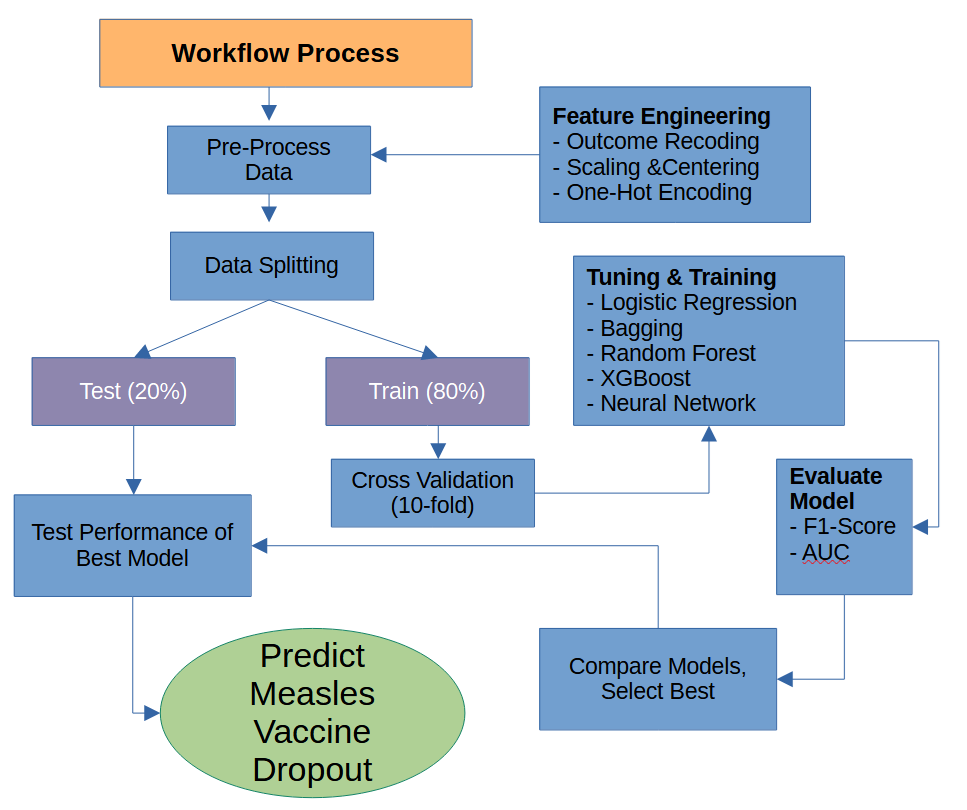
\includegraphics[width=6.47917in,height=\textheight]{workflow.png}

}

\caption{\textbf{Figure 1. Our Machine Learning Workflow Process}}

\end{figure}%

\subsubsection{\texorpdfstring{\emph{Feature
Selection}}{Feature Selection}}\label{feature-selection}

We chose 10 features from the MICS survey to represent the contextual
factors that drive measles vaccine dropout such as household
characteristics (e.g., access to electricity and running water, house
construction materials ), family socieconomics (e.g., wealth score
calculated by MICS) , mother's education level, and family participation
in national immunization campaigns. Moreover, there were four national
immunization campaigns in the country and the MICS asked respondents to
identify which event they attended. For illustration purposes we
collapsed these four variables into one and coded it as attending one
event (e.g., some), two or three events (e.g., half), or all four events
(e.g., all) which can be seen on the x-axis in Figure 2, in addition to
rural vs urban, and mother's education level as they relate to the
target variable. We can see from this figure that the rural-urban divide
is important for understanding the outcome alongside mother's education
level which seems to correlate with participation in the immunization
campaigns.

The MICS contains information about which province children live in;
therefore, we were able to leveraged
\href{https://www.worldbank.org/en/data/interactive/2019/08/01/afghanistan-interactive-province-level-visualization}{World
Bank} indicators for each Afghan province to provide additional
geographic contextual features. This province indicators include
conflict score with values closer to 100 indicating extreme instability
from armed conflict, female literacy rate, health infrastructure with
scores closer to 100 indicating greater delivery of medical goods to the
public, population density, and poverty rate. Table 1 presents features
used to predict the target outcome. We present in Figure 3 the breakdown
in the target variable distributed across the provinces as well as show
health institution availability and female literacy rates. We can see
variation in the provinces across these indicators and our outcome
variable. Overall we had 22 features in total to predict the target
variable.

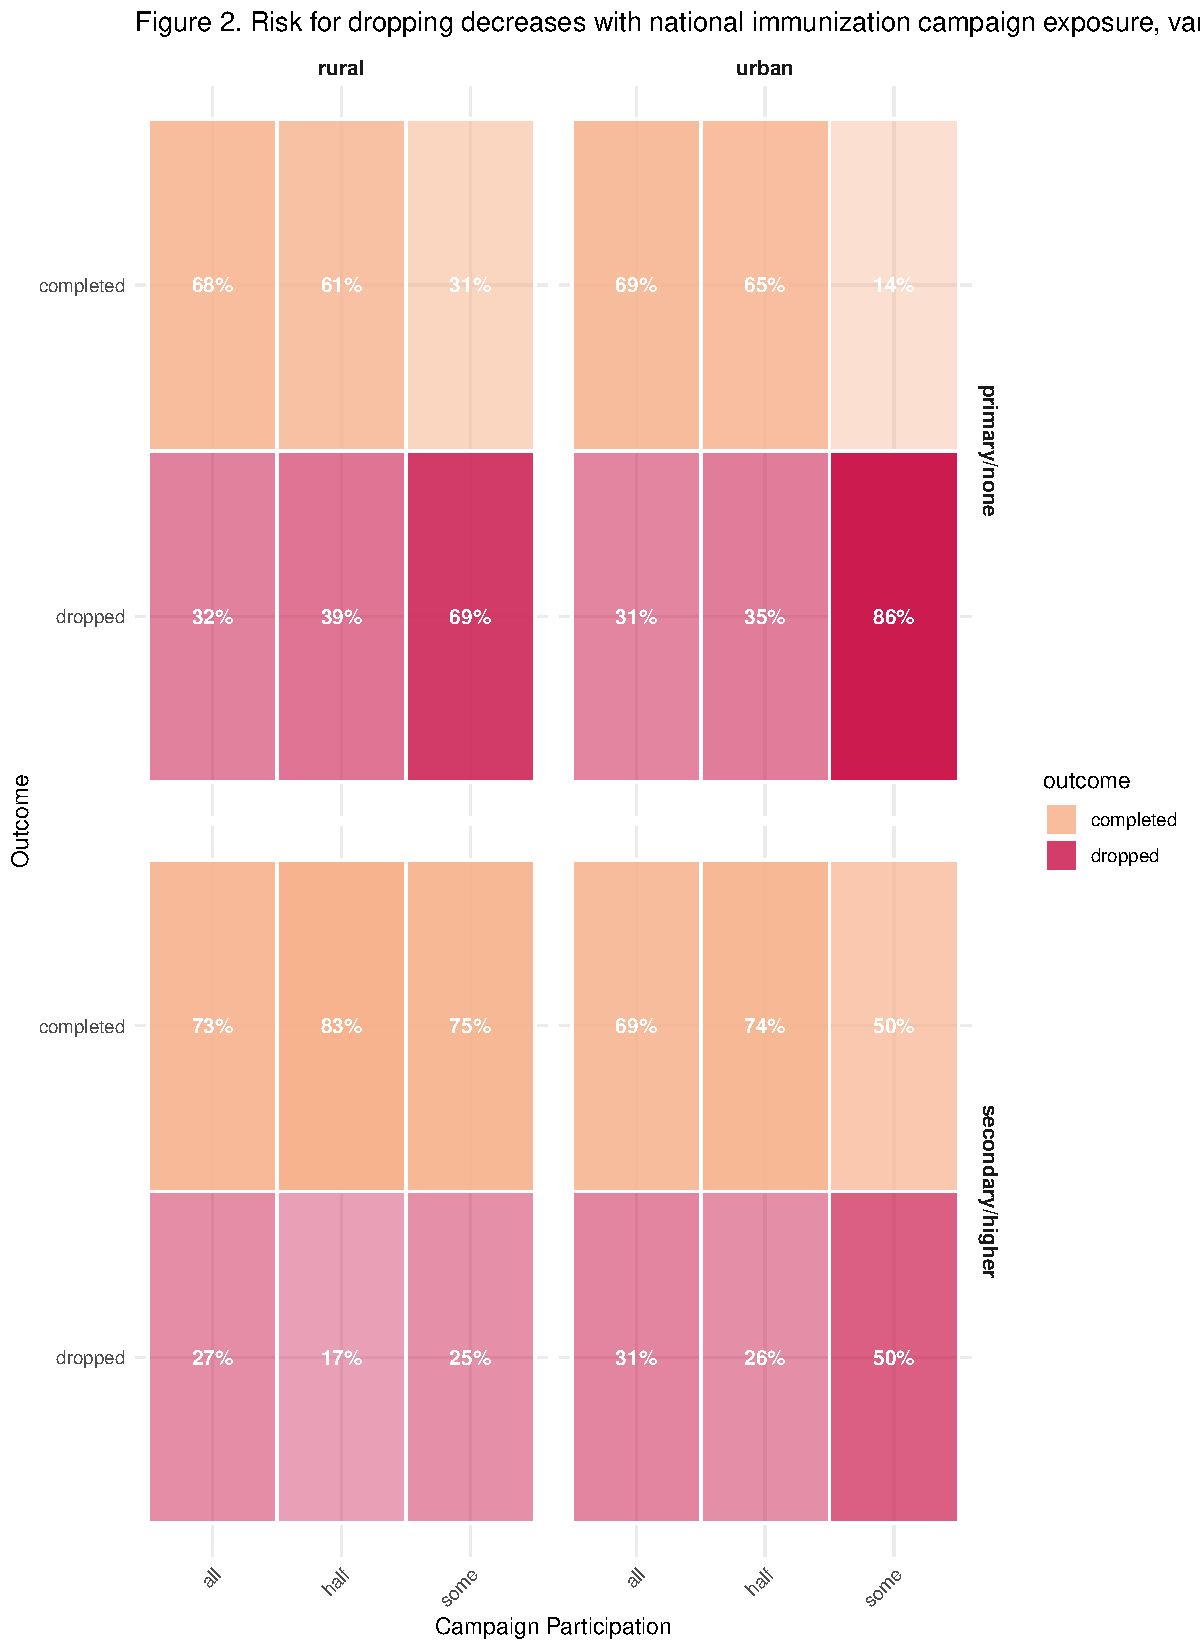
\includegraphics{mmr_dropout_ml_paper_files/figure-pdf/unnamed-chunk-2-1.pdf}

\begin{longtable}[]{@{}
  >{\raggedright\arraybackslash}p{(\columnwidth - 2\tabcolsep) * \real{0.3614}}
  >{\raggedright\arraybackslash}p{(\columnwidth - 2\tabcolsep) * \real{0.6386}}@{}}
\caption{Features Used For Predicting Measles Vaccine
Dropout}\tabularnewline
\toprule\noalign{}
\begin{minipage}[b]{\linewidth}\raggedright
variable
\end{minipage} & \begin{minipage}[b]{\linewidth}\raggedright
label
\end{minipage} \\
\midrule\noalign{}
\endfirsthead
\toprule\noalign{}
\begin{minipage}[b]{\linewidth}\raggedright
variable
\end{minipage} & \begin{minipage}[b]{\linewidth}\raggedright
label
\end{minipage} \\
\midrule\noalign{}
\endhead
\bottomrule\noalign{}
\endlastfoot
hh6 & Area \\
im12a & Participate in campaign, national immunization day A \\
im12b & Participate in campaign, national immunization day B \\
im12c & Participate in campaign, national immunization day C \\
im12d & Participate in campaign, national immunization day D \\
melevel & Mother's education \\
wscore & Combined wealth score \\
hh52 & Number of children age 5-17 \\
hc3 & Number of Room in House \\
hc4 & Main material of floor \\
hc7g & Household have: A Mattress \\
hc8 & Household have electricity \\
hc14 & Household owns the dwelling \\
ws1 & Main source of drinking water \\
ws9 & Treat water to make safer for drinking \\
ws11 & Type of toilet facility \\
hw3 & Soap or detergent present at place of handwashing \\
conflict\_index & \\
female\_literacy\_rate & \\
health\_institutional\_delivery & \\
density\_per\_inhabited\_area & \\
poverty\_rate & \\
outcome & \\
\end{longtable}

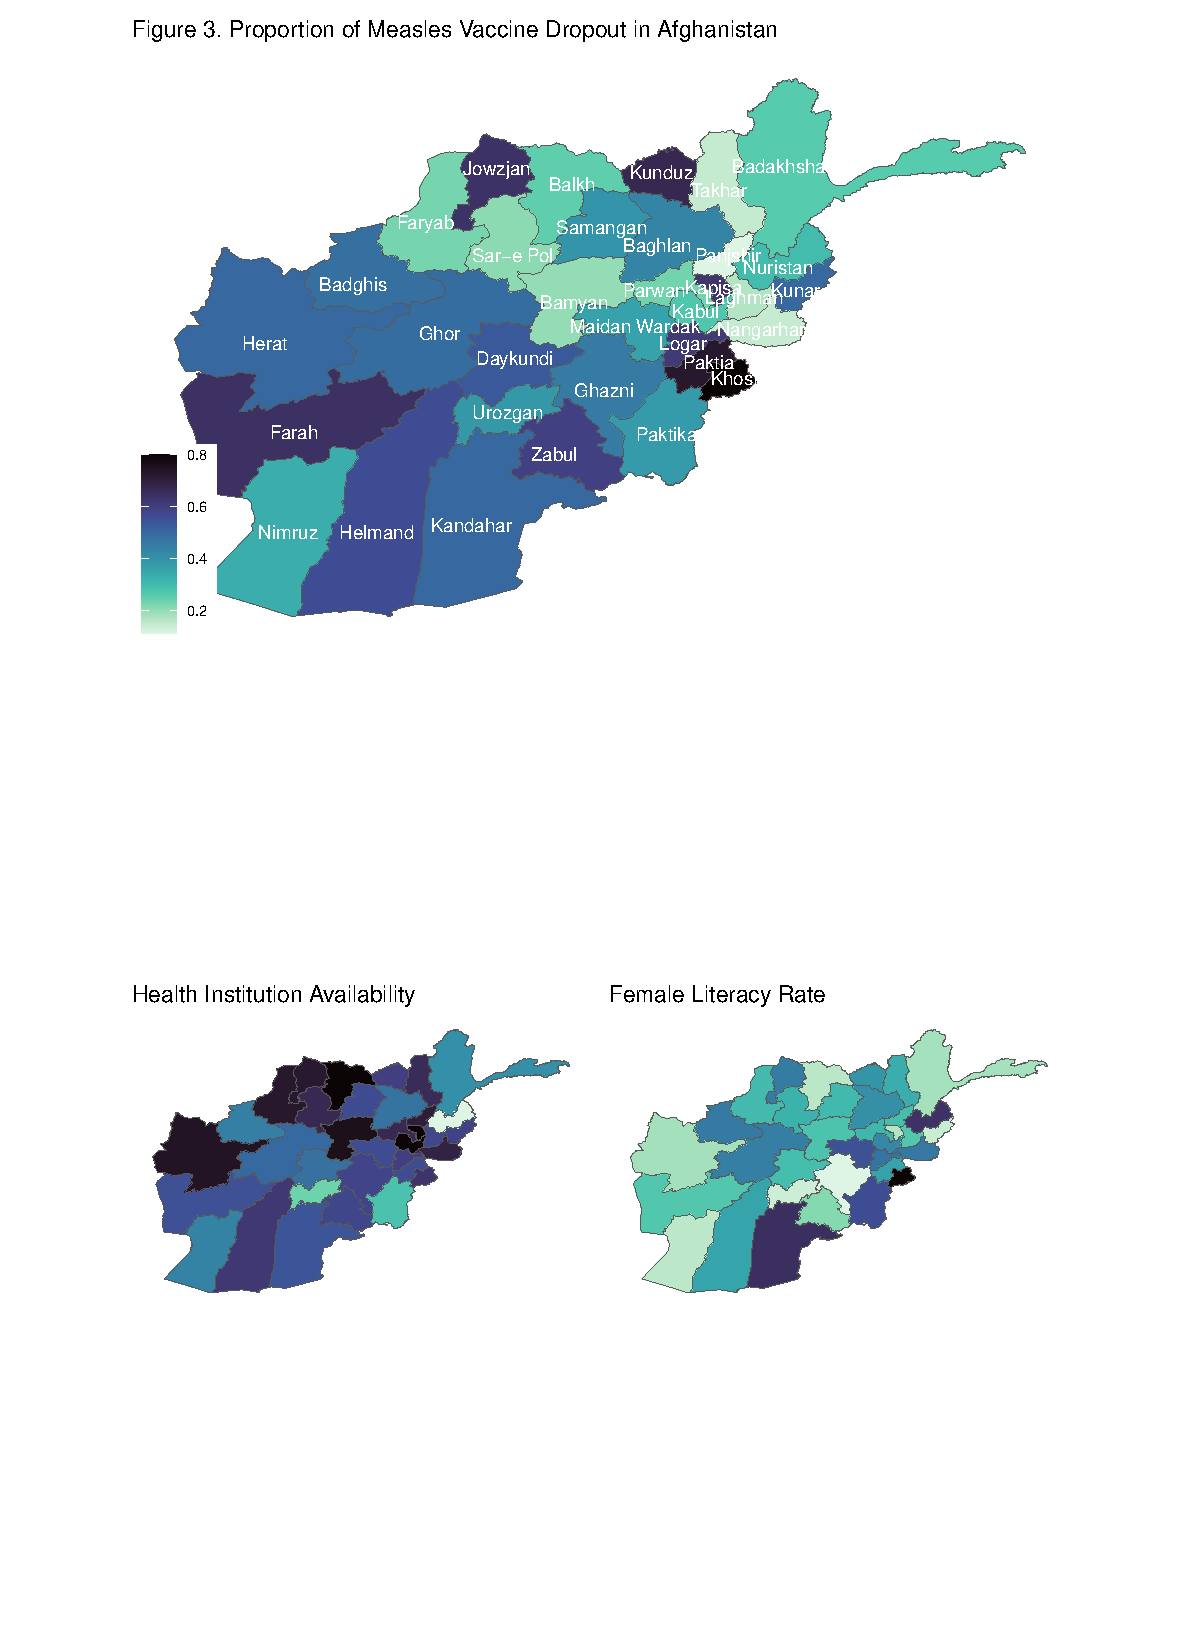
\includegraphics{mmr_dropout_ml_paper_files/figure-pdf/unnamed-chunk-2-2.pdf}

\subsubsection{}\label{section}

\subsubsection{\texorpdfstring{\emph{Feature
Engineering}}{Feature Engineering}}\label{feature-engineering}

Across our factor features we collapsed levels when appropriate, such as
when very few cases were observed in obscure levels. For instance, very
few mothers in the survey had a secondary or higher education (e.g.,
\textless{} 14 percent) and therefore we collapsed all levels secondary
and above together. Alternatively, very few had no formal education and
we collapsed this level with primary education. Access to water feature
factor levels were collapsed into city, well, or other as well as access
to plumbing levels were collapsed into sewer, septic, pit, outhouse,
latrine, and other. One shot encoding was used for factor levels and
quantitative variables such as the family wealth score and province
indicators were scaled and centered.

\section{Results}\label{results}

For computation we used the r-language and conducted all of our modeling
using tidymodels. We tuned hyperparameters using cross validation during
model training and choose models with the best AUC and F1-scores. We
start with the logistic regression as a base learner to compare against
ensemble methods that require parameter tuning. We show parameter tuning
values in Figures 4 and 5 for all five models.

The logistic regression was only tuned for the penalty parameter and was
the less demanding algorithm to compute. Bagging was tuned for cost
complexity between .00001 and .001, minimum number of n (e.g., 8, 10, 12
shown as columns in Figure 4), and tree depth between 2 to 6. Random
forest was tuned for number of mtry to use between 3 to 10 (e.g., ),
minimum n between 8 to 16 (e.g., shown as columns in Figure 4), and
number of trees (e.g., 500, 1000, 1500, 2000). Neural networks using the
nnet engine we tuned parameters penalty (i.e., amount of regularization,
epochs, and hidden units). For this model we used the
\texttt{dials::grid\_space\_filling()} function which is used to
construct parameter grids that try to cover the parameter space in a way
that the parameter space does not have observed combinations that are
close to one another. This resulted in 300 combinations to use for
tuning and can be seen in Figure 5. The XGBoost had the most parameters
to tune and again we relied on \texttt{dials::grid\_latin\_hypercube()}
which achieves something similar to that what we used in the neural
network. This allowed us to tune tree depth, minimum node size, number
of trees, minimum loss reduction, sample size (e.g., proportion
observation samples, mtry, and learning rate resulting in training with
500 combinations of these parameters shown in Figure 5.

\newpage

Figure 4. Hyperparameter Tuning for ML Model Training

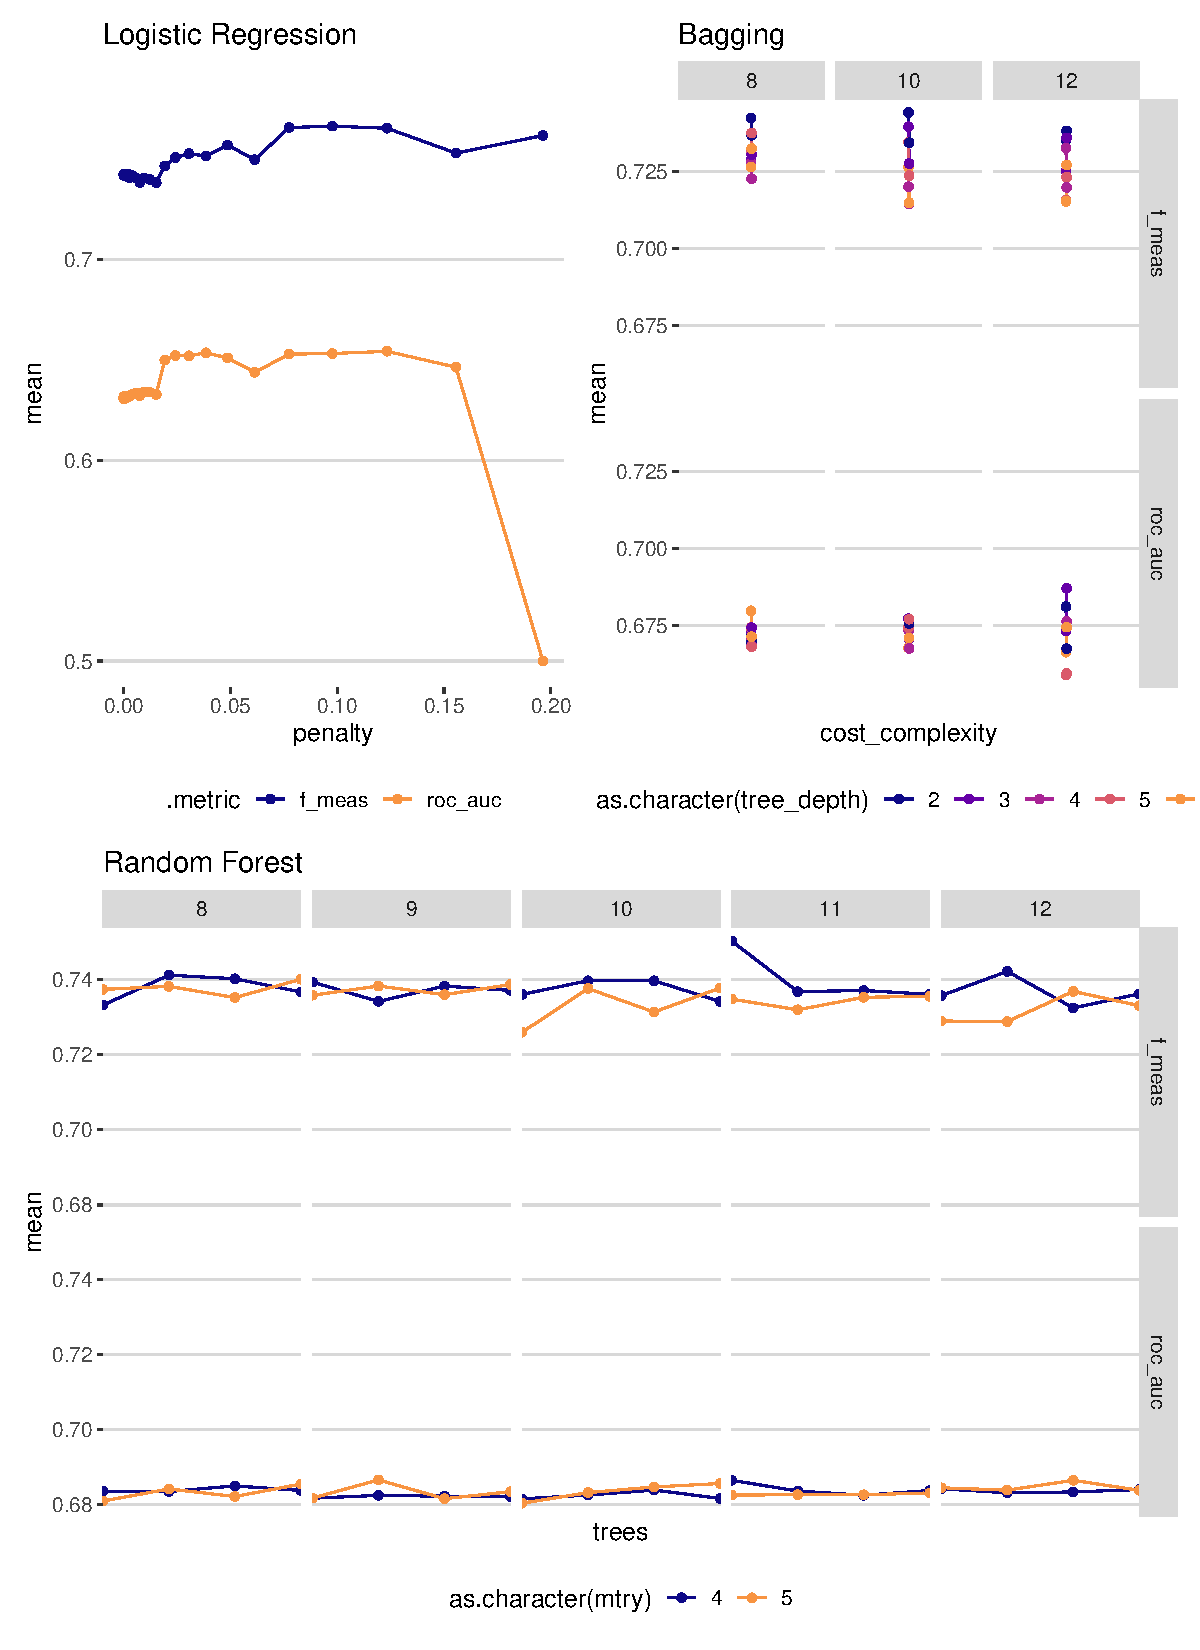
\includegraphics{mmr_dropout_ml_paper_files/figure-pdf/unnamed-chunk-4-1.pdf}

\newpage

Figure 5. Continuation of Hyperparameter Tuning for ML Model Training

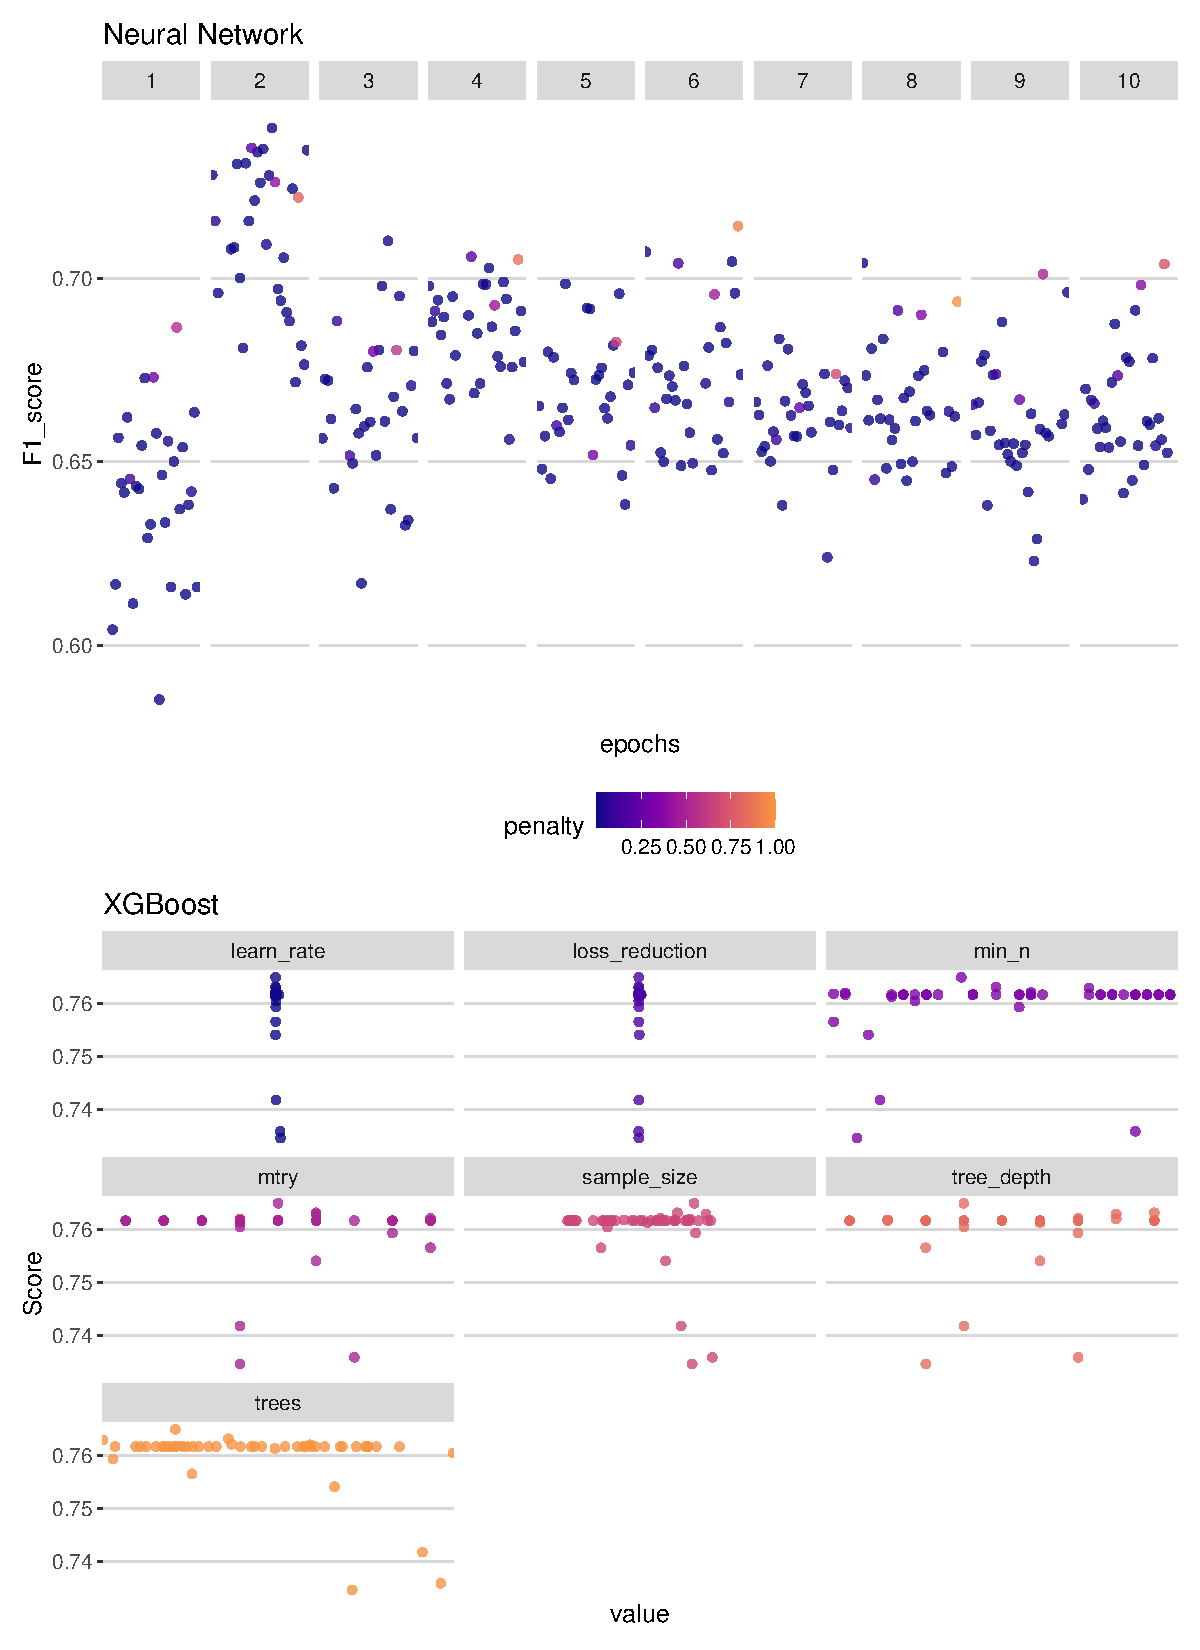
\includegraphics{mmr_dropout_ml_paper_files/figure-pdf/unnamed-chunk-5-1.pdf}

Once we picked our best models for each algorithm based on F1-scores and
the AUC we applied the best model to the test set and predicted measles
vaccine dropout for each one. We present performance metrics for each
final model on the test set in Figure 6. All of the models were very
close in performance yet we chose the neural network model because it
performed the best on the F1-score (.722) yet came in second place after
random forest on AUC (.633). These scores are not great but they do
better than random chance. Figure 7 presents the most important
variables for interpretability purpose.

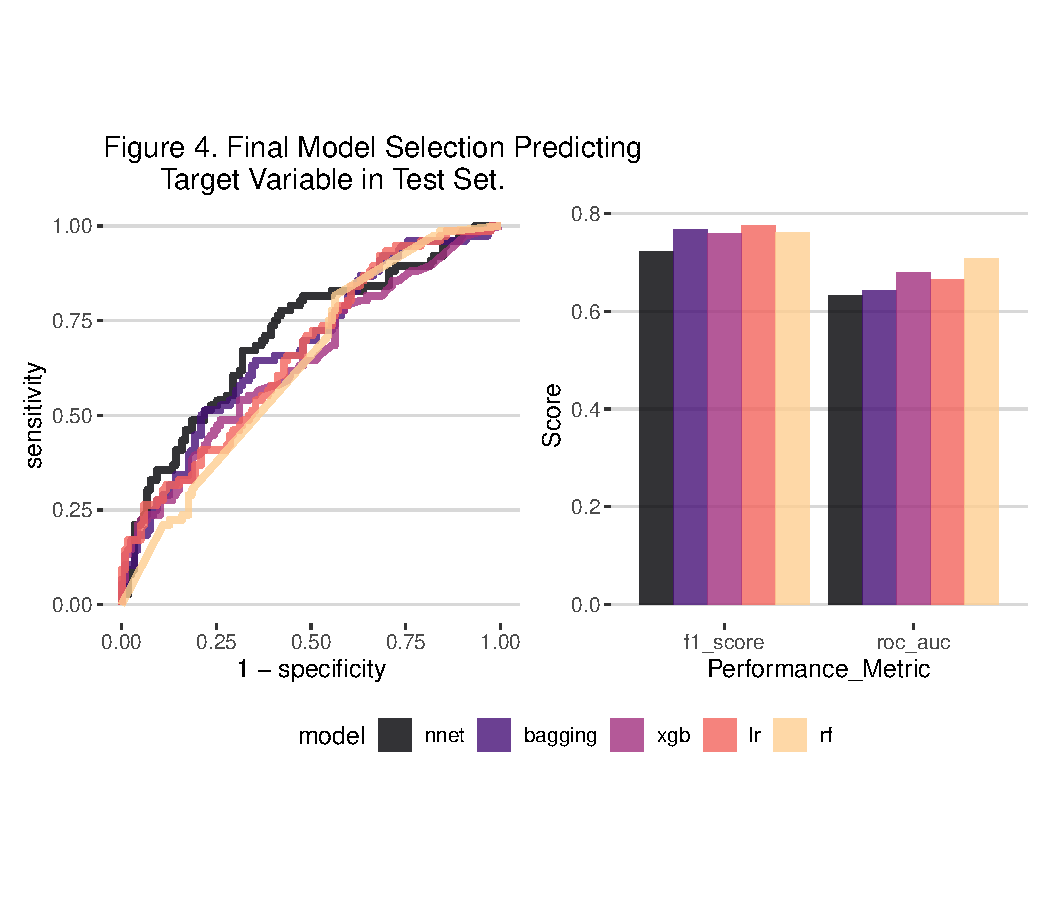
\includegraphics{mmr_dropout_ml_paper_files/figure-pdf/unnamed-chunk-6-1.pdf}

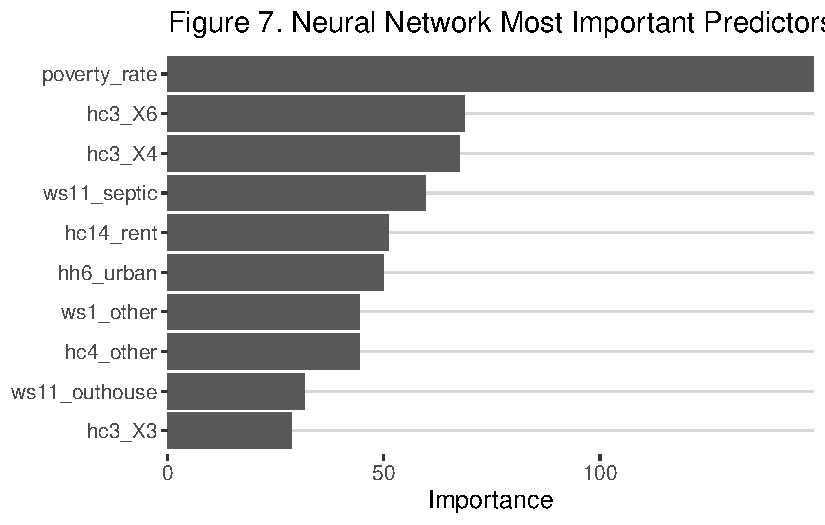
\includegraphics{mmr_dropout_ml_paper_files/figure-pdf/unnamed-chunk-7-1.pdf}

\section{Discussion}\label{discussion}

This study aimed to predict measles vaccination dropout among Afghan
children using machine learning with 2023 MICS and World Bank data. We
found the neural network model performed best, exceeding random chance
but with moderate performance. This highlights the challenge of
predicting dropout in this complex setting. Key predictors identified by
the model, such as provincial population density, number of rooms per
house, having a septic tank, and renting home. These findings underscore
the multifaceted nature of vaccination dropout. While imperfect, the
models offer a valuable tool for public health efforts. These can help
identify at-risk children and regions, they can assist in targeting
limited resources and interventions more effectively, address factors
like health service access, and campaign outreach.

Limitations include reliance on the small samples size of almost 1,000
respondents, necessary feature simplification such as collapsing
factors, and a reliance on tool parameter specification for for model
tuning. Future work could explore richer data sources or refined
modeling techniques. In conclusion, this research demonstrates the
utility of machine learning for identifying children at risk of measles
vaccination dropout in Afghanistan. The models, despite limitations,
provide actionable insights to guide targeted public health strategies
aimed at improving crucial two-dose vaccination coverage.




\end{document}
